
%___________________________________________________________________
% Load Class
% beamer will auto load: hyperref, color, xcolor, amsthm

\documentclass[
  fontsize=10pt, 
  aspectratio=169,
  xcolor={dvipsnames}
]{beamer}


%___________________________________________________________________
% Load Packages
% inputenc is redundant for modern LaTeX versions.
% fontenc should only be used if the font supports T1 encoding.

\usepackage{fontspec}               % required for system fonts
\usepackage{microtype}              % better typography
\usepackage{polyglossia}            % languages

% \usepackage{enumitem}

% citations
\usepackage[
  backend=biber,              
  style=ieee,                 
]{biblatex}   
\usepackage[
  autostyle=true, 
  german=quotes
]{csquotes}

% better unit display
\usepackage[
  locale=DE,
  mode=match,
  % per-mode-fraction,
  range-units=repeat,
  range-phrase={{~bis~}}
]{siunitx}

\usepackage{amsmath}

% input external data
\usepackage{listings}
\usepackage{graphicx} 
\usepackage{svg}
\usepackage{animate}

% improve visualization of data
\usepackage{booktabs}
\usepackage{tabularx}
\usepackage{longtable}
\usepackage{subcaption}	

\usepackage{appendixnumberbeamer}

\usetheme[]{metropolis}     % beamer style


%___________________________________________________________________
% Dimensions

\newlength{\imagewidth}
\setlength{\imagewidth}{1\columnwidth}

\newlength{\imageheight}
\setlength{\imageheight}{0.85\textheight}

%___________________________________________________________________
% Colors

\definecolor{colorblue}{HTML}{0480CC}				% color for weblinks
\definecolor{colordarkblue}{HTML}{4C1DCC}			% no use case at the moment
\definecolor{colorgreen}{HTML}{26CC1B}				% color for citations
\definecolor{colorred}{HTML}{CC1204}				% color for pdf links
\definecolor{coloryellow}{HTML}{F0B707}			    % color for warnings

%___________________________________________________________________
% New Makros

\newcommand{\imagesource}[1]{\par\footnotesize\textbf{Quelle:}~#1}   	%   Quellen für Bilder
\newcommand{\imagelegend}[1]{\par\footnotesize\textbf{Legende:}~#1}

\newcommand{\missing}{%
    \textcolor{coloryellow}{MISSING}%
    \PackageWarning{JHstyle}{You used the 'missing' macro at this line. Remove it before finalising document}%
}
\newcommand{\improve}{%
    \textcolor{coloryellow}{IMPROVE}%
    \PackageWarning{JHstyle}{You used the 'improve' macro at this line. Remove it before finalising document}%
}

%___________________________________________________________________
% Renamings

% \renewcommand{\lstlistingname}{Quellcode}						%	Snippet umbenennen
% \renewcommand{\lstlistlistingname}{Codeverzeichnis}	

\addto\captionsgerman{%
  \renewcommand{\proofname}{Beweis}
}

% \renewcommand{\mkcitation}[1]{#1}

%___________________________________________________________________
% Commands

\setdefaultlanguage{german}
\setotherlanguage{english}

% \addbibresource{sources.bib}

\graphicspath{{media/}}  

\hypersetup{
  % hidelinks,
  colorlinks=true,
  linkcolor=.,
  anchorcolor=.,
  citecolor=colorgreen,
  filecolor=magenta,      
  urlcolor=colorblue,
  bookmarksnumbered=true,
  breaklinks=true,
  pdfauthor=Jan Hoegen,
  pdftitle=Vorstellung der Automatisierungstechnik,
}


%___________________________________________________________________
% Ttile Page

\title{Vertiefung Automatisierungstechnik}
\subtitle{Elektro- und Informationstechnik Bachelor}
\date{\today}
\author{Jan Hoegen}
\institute{
    Fachschaft EIT\\
    Hochschule Karlsruhe\\
}
% \setbeamertemplate{frame footer}{EITB AUT. Jan Hoegen}


%___________________________________________________________________
% Document

\begin{document}
    \maketitle

    % \begin{frame}{Inhaltsverzeichnis}
    % \setbeamertemplate{section in toc}[sections numbered]
    % \tableofcontents[hideallsubsections]
    % % \tableofcontents
    % \end{frame}

    
\begin{frame}{Überischt der Studienverlaufs}
    \begin{figure}
        \centering
        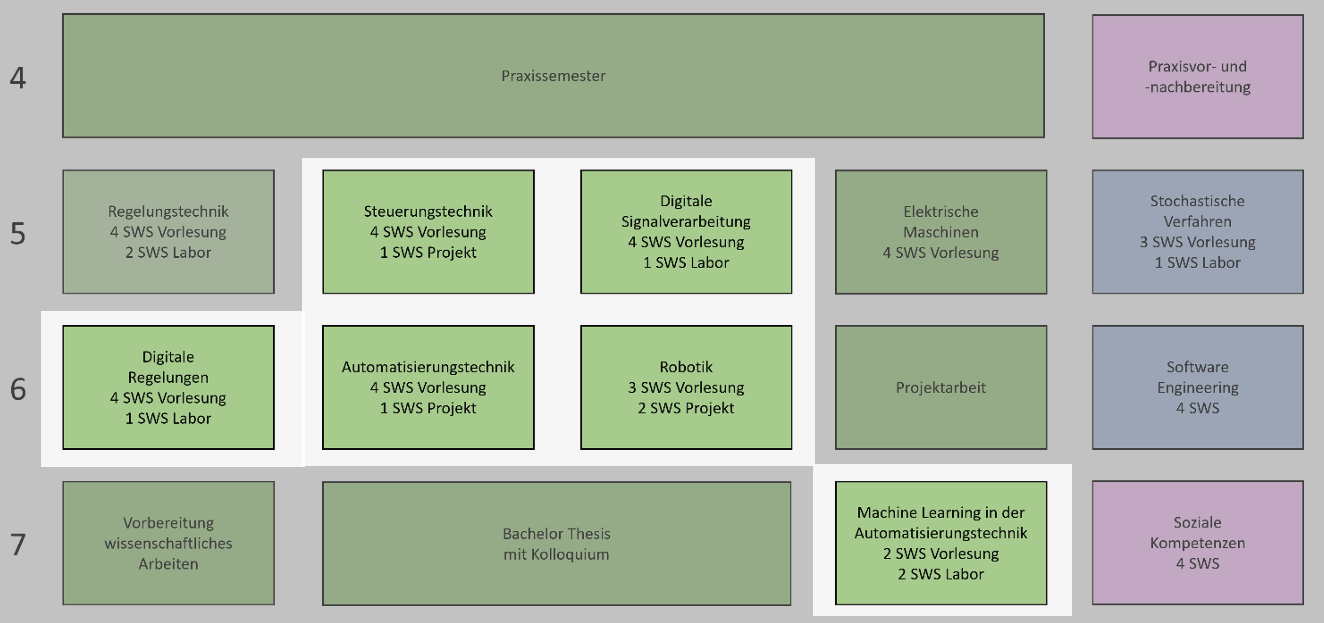
\includegraphics[width=\imagewidth, height=0.95\imageheight, keepaspectratio]{übersicht grayed}
        \caption{Modulüberischt Automatisierungstechnik.}
    \end{figure}
\end{frame}
    %___________________________________________________________________

\begin{frame}{Steuerungstechnik (Nenninger)}
\begin{columns}[T, totalwidth=\textwidth]

\begin{column}{0.5\textwidth}
    
\textbf{Inhalte}
\begin{itemize}
    \item SPS Programmierung
    \item Zustandsgraphen und Schaltnetze
    \item Kodiersysteme
    \item Integration von Sensoren und Aktoren
\end{itemize}

\vspace{0.3cm}
\textbf{Rahmendaten}
\begin{description}
    \item[Klausur] leicht
    \item[Vorlesung] leicht 
    \item[Labor] zeitaufwendig
\end{description}

\end{column}

\begin{column}{0.45\textwidth}
\begin{figure}
    \centering
     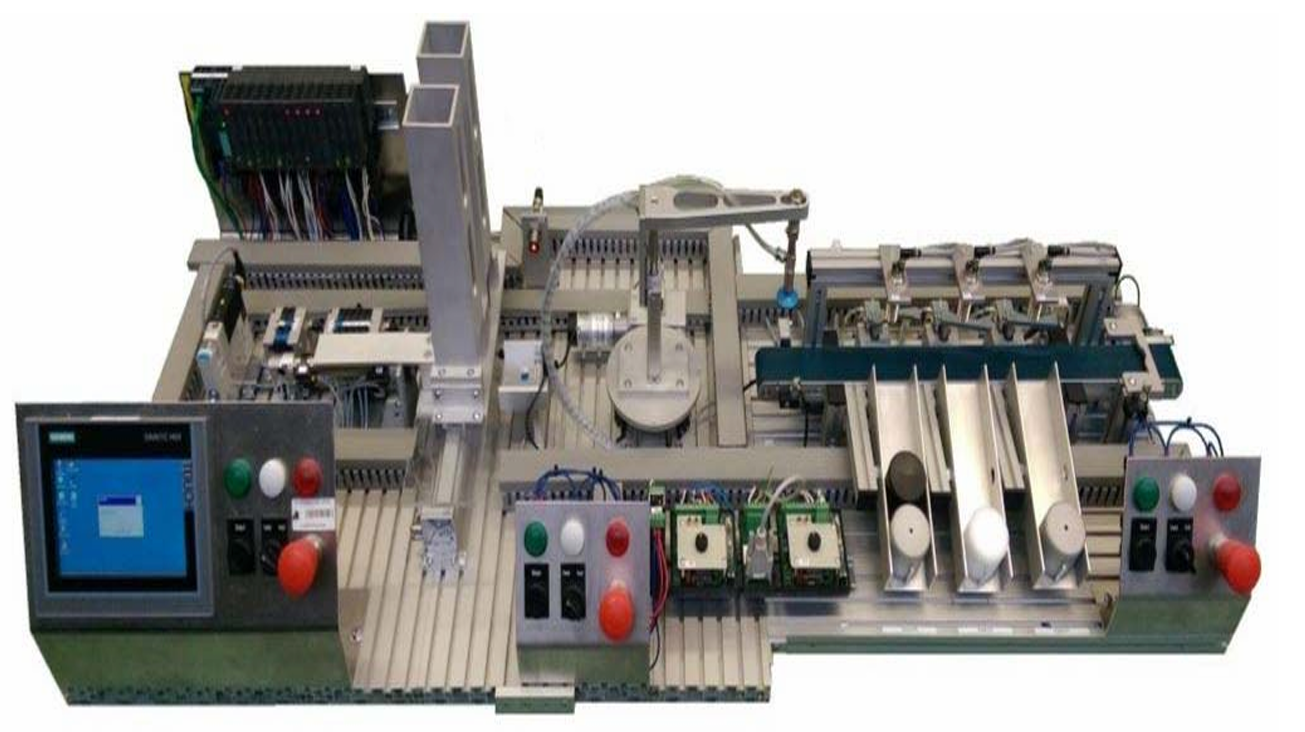
\includegraphics[width=\imagewidth, height=0.8\imageheight, keepaspectratio]{siemens}
    \caption{S7 Anlage Dosensortierer.}
\end{figure}
\end{column}

\end{columns}

\end{frame}


%___________________________________________________________________

\begin{frame}{Automatisierungstechnik (Nenninger)}
\begin{columns}[T, totalwidth=\textwidth]

\begin{column}{0.5\textwidth}

\textbf{Inhalte}
\begin{itemize}
    \item Modellbildung technischer Prozesse
    \item Grafische, mathematische Modelle
    \item Feldbus- und Kommunikationssysteme
    \item Zuverlässigkeit, Sicherheit und Verfügbarkeit
    \item Prozessführung, SCADA
\end{itemize}

\vspace{0.3cm}
\textbf{Rahmendaten}
\begin{description}
    \item[Klausur] leicht
    \item[Vorlesung] leicht
    \item[Labor] enorm aufwendig
\end{description}

\end{column}

\begin{column}{0.45\textwidth}
\begin{figure}
    \centering
     \includegraphics[width=\imagewidth, height=0.95\imageheight, keepaspectratio]{ballon}
    \caption{Station Luftballon.}
\end{figure}
\end{column}

\end{columns}

\end{frame}


%___________________________________________________________________

\begin{frame}{Digitale Regelungssysteme (Feßler)}

\textbf{Inhalte}
\begin{itemize}
    \item Digitale Regelungssysteme im zeitdiskreten und $z$-Bereich
    \item Entwurf und Erweiterung von PID-Reglern
    \item Robustheit, Sensitivität, Wasserbett-Effekt
    \item Modellgestützte Verfahren: IMC, MPC, Youla-Parametrierung
    \item Mehrschleifige Regelungen und Prozessführung
    \item Fuzzy Control und digitale Signalverarbeitung
    \item Implementierung auf Signalprozessoren
\end{itemize}

\vspace{0.3cm}
\textbf{Rahmendaten}
\begin{description}
    \item[Klausur] sehr schwer
    \item[Vorlesung] schwer
    \item[Labor] ?
\end{description}

\end{frame}


%___________________________________________________________________

\begin{frame}{Digitale Signalverarbeitung (Strohrmann)}
\begin{columns}[T, totalwidth=\textwidth]

\begin{column}{0.5\textwidth}

\textbf{Inhalte}
\begin{itemize}
    \item Abtasttheorem und diskrete Signale
    \item z-Transformation und Fourier-Analyse
    \item FIR- und IIR-Filterentwurf
    \item DFT und FFT-Algorithmen
    \item Echtzeit-Signalverarbeitung auf DSPs
\end{itemize}

\vspace{0.3cm}
\textbf{Rahmendaten}
\begin{description}
    \item[Klausur] mittel
    \item[Vorlesung] mittel 
    \item[Labor] mittel
\end{description}

\end{column}

\begin{column}{0.45\textwidth}
\begin{figure}
    \centering
     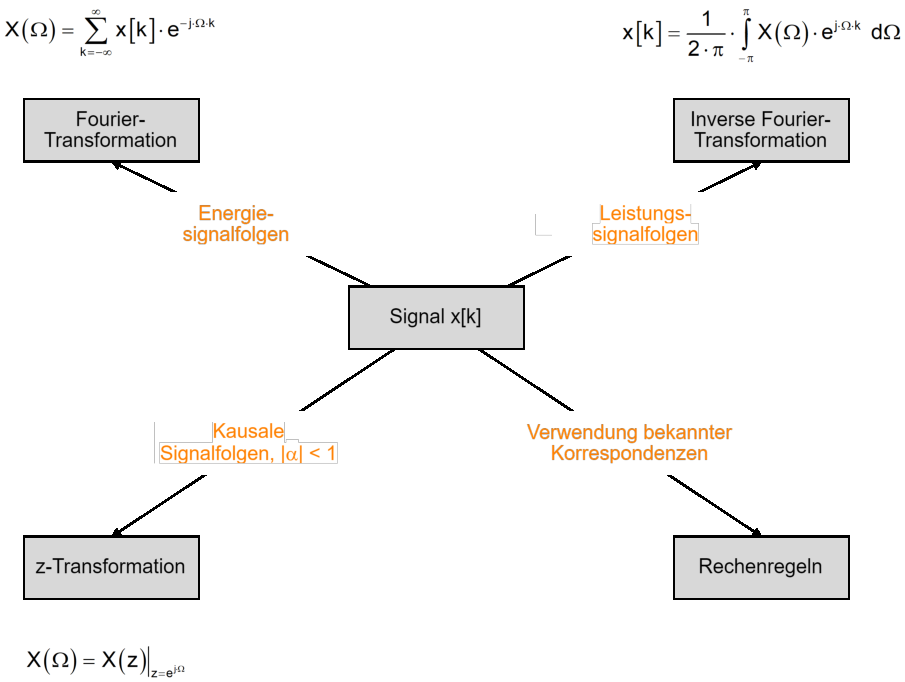
\includegraphics[width=\imagewidth, height=0.8\imageheight, keepaspectratio]{signal}
    \caption{Signaltransformationen.}
\end{figure}
\end{column}

\end{columns}

\end{frame}


%___________________________________________________________________

\begin{frame}{Robotik (Braun)}
\begin{columns}[T, totalwidth=\textwidth]

\begin{column}{0.5\textwidth}

\textbf{Inhalte}
\begin{itemize}
    \item Kinematik und Koordinatentransformationen
    \item Bahnplanung und Bewegungsprofile
    \item Sensorik und Roboterarchitekturen
    \item Programmierung von Robotersystemen
\end{itemize}

\vspace{0.3cm}
\textbf{Rahmendaten}
\begin{description}
    \item[Klausur] leicht
    \item[Vorlesung] leicht 
    \item[Labor] leicht
\end{description}

\end{column}

\begin{column}{0.45\textwidth}
\begin{figure}
    \centering
     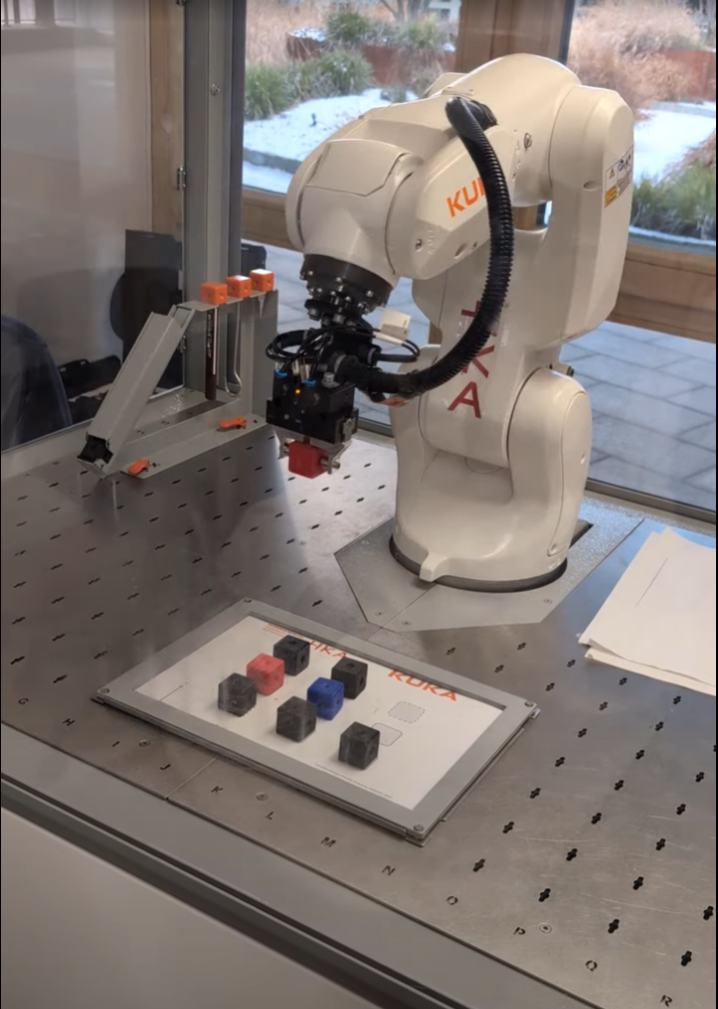
\includegraphics[width=\imagewidth, height=0.95\imageheight, keepaspectratio]{roboter}
    \caption{Ein Roboter.}
\end{figure}
\end{column}

\end{columns}

\end{frame}


%___________________________________________________________________

\begin{frame}{Machine Learning in der Automatisierungstechnik (Nenninger)}
\begin{columns}[T, totalwidth=\textwidth]

\begin{column}{0.5\textwidth}

\textbf{Inhalte}
\begin{itemize}
    \item Prozessleitsysteme
    \item Prozesskomponenten SCADA, MES
    \item Datenspeicherung und Cloud-/Datenbankanbindung
    \item Schnittstellen: MQTT, OPC, OPC UA
    \item Grundlagen des Machine Learning für Prozessdaten
\end{itemize}

\vspace{0.3cm}
\textbf{Rahmendaten}
\begin{description}
    \item[Klausur] leicht
    \item[Vorlesung] leicht
    \item[Labor] leicht
\end{description}

\end{column}

\begin{column}{0.45\textwidth}
\begin{figure}
    \centering
     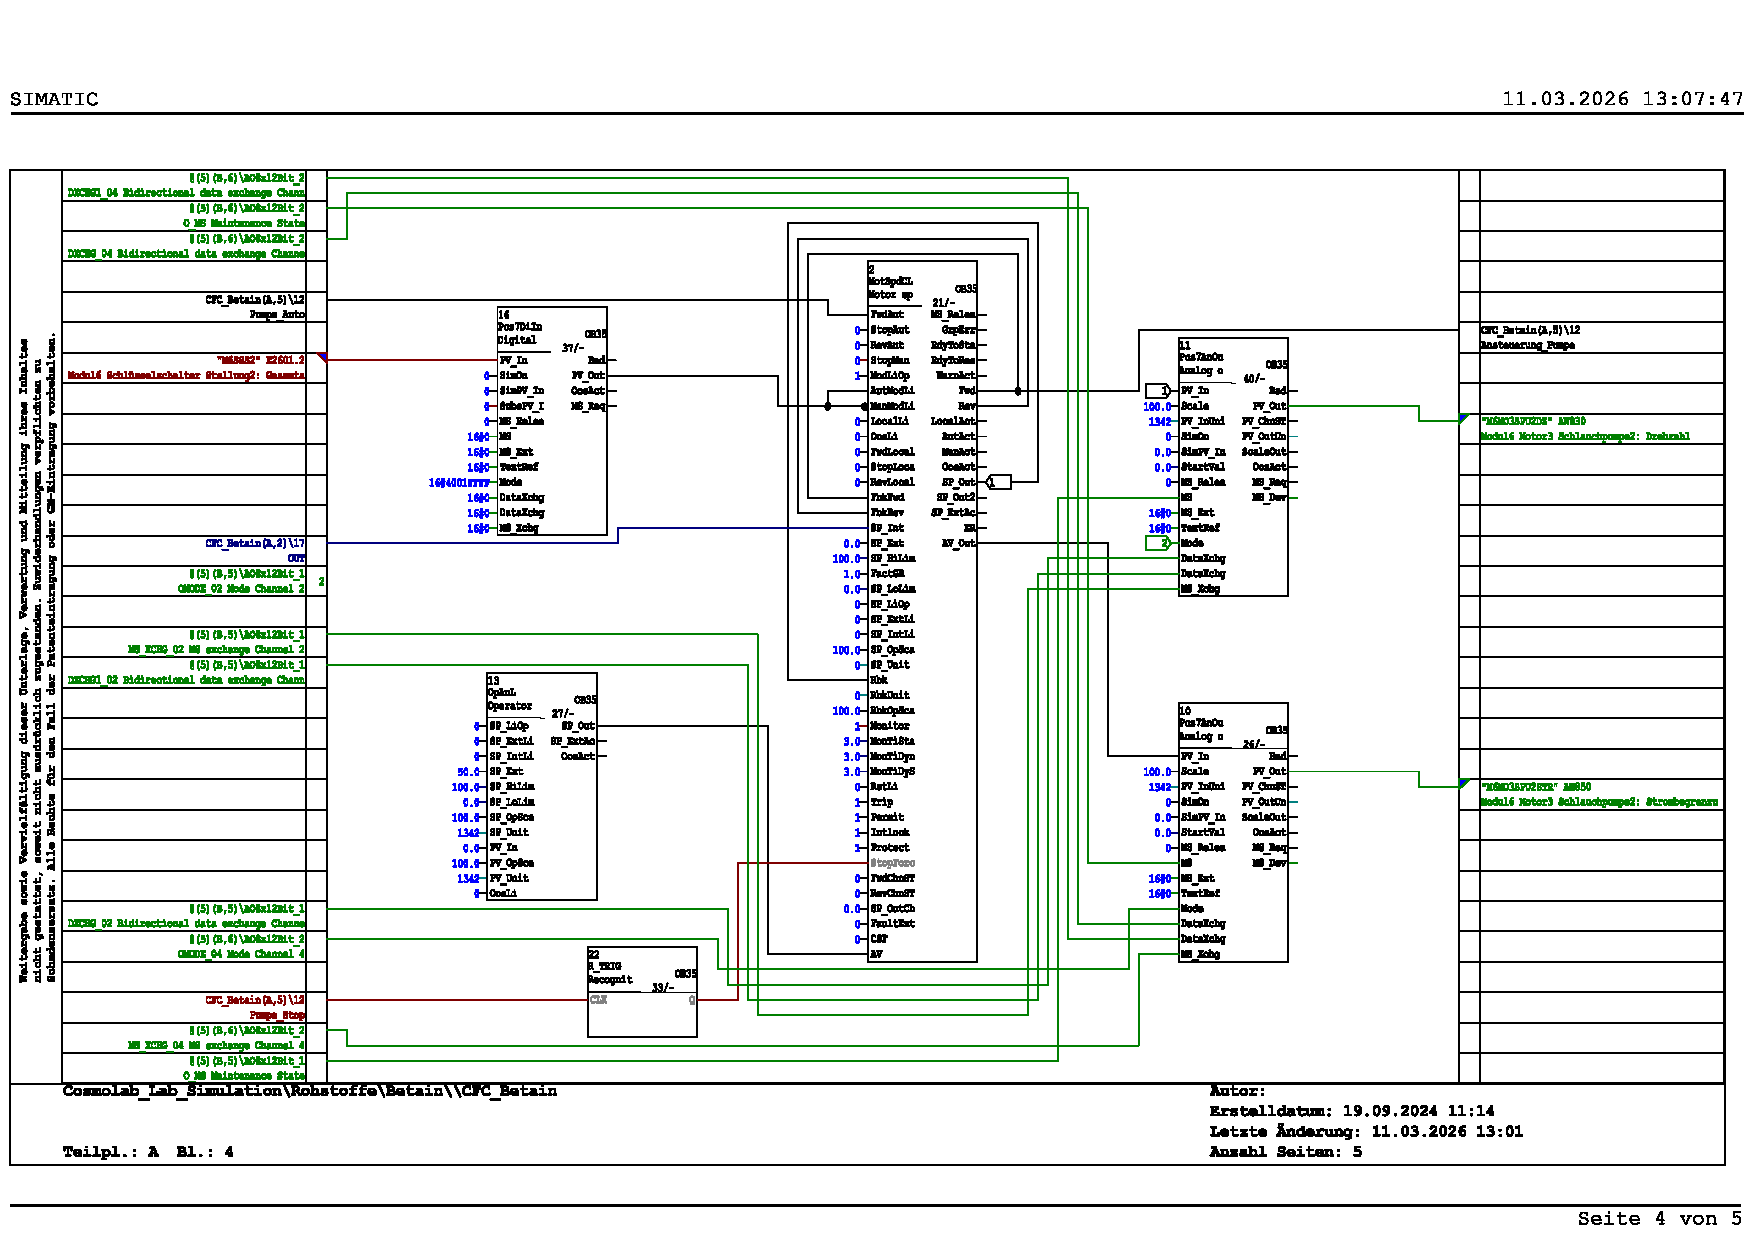
\includegraphics[width=\imagewidth, height=0.95\imageheight, keepaspectratio]{betain}
    \caption{Prozessmodell Betainpumpe.}
\end{figure}
\end{column}

\end{columns}
\end{frame}

\end{document}